% !TeX root = ../main.tex

\appendix{A}{實際操作介面}
本附錄展示了本研究概念實作的部分功能截圖。
\section{AID錢包}
\begin{figure}
  \centering
  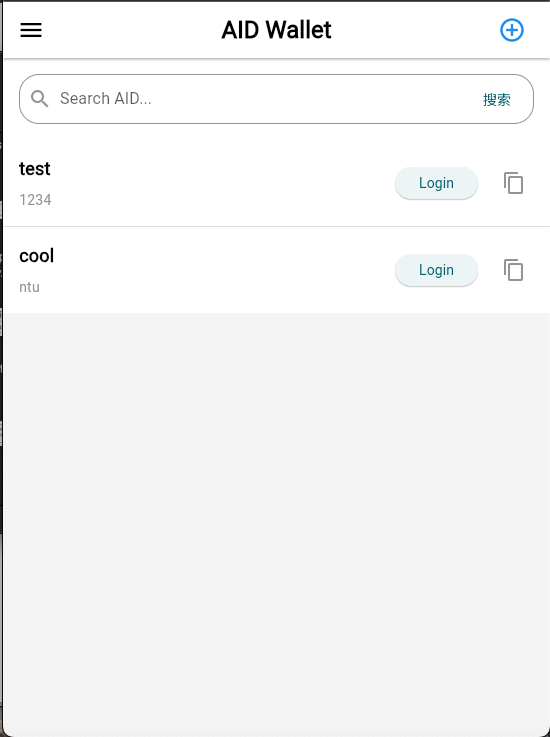
\includegraphics[width=\linewidth]{figures/wallet-demo.png}
  \caption{AID錢包}
  \label{fig:appendix-wallet}
\end{figure}
\clearpage
\begin{figure}[p]
  \centering
  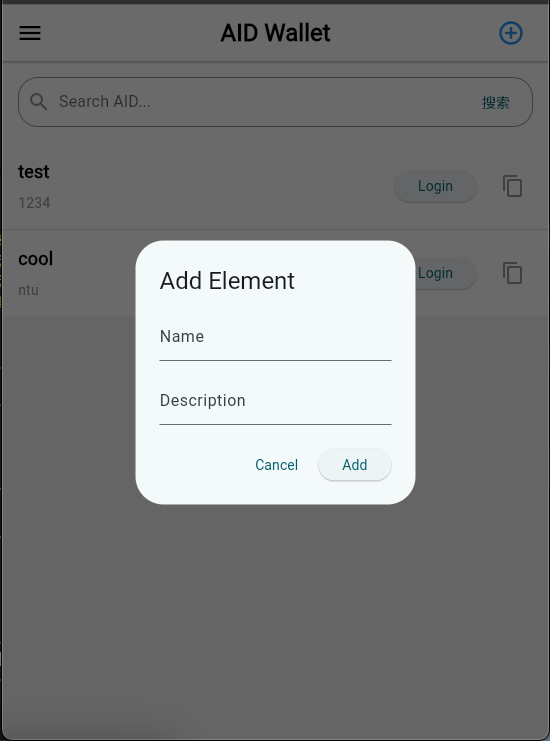
\includegraphics[width=\linewidth]{figures/wallet-create-demo.png}
  \caption{本地身份創建}
  \label{fig:appendix-wallet-create-demo}
\end{figure}
\clearpage
\begin{figure}[p]
  \centering
  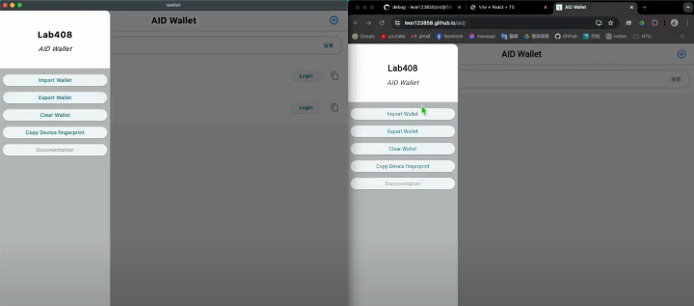
\includegraphics[width=\linewidth]{figures/wallet-drawer-demo.png}
  \caption{錢包遷移}
  \label{fig:appendix-wallet-drawer-demo}
\end{figure}
本節展示實作部分的AID錢包操作介面。
\begin{itemize}
  \item 圖\ref{fig:appendix-wallet}展示了AID錢包的實際操作介面。使用者可以通過錢包進行身分創建、身份管理等操作。
  \item 圖\ref{fig:appendix-wallet-create-demo}展示了本地身份創建的操作流程。使用者可以通過錢包創建本地身份,並設置密碼保護。
  \item 圖\ref{fig:appendix-wallet-drawer-demo}展示了錢包遷移的操作流程。使用者可以通過錢包將本地身份遷移到其他設備上,實現身份的跨設備管理。
\end{itemize}
\section{AI聊天軟體}
\begin{figure}
  \centering
  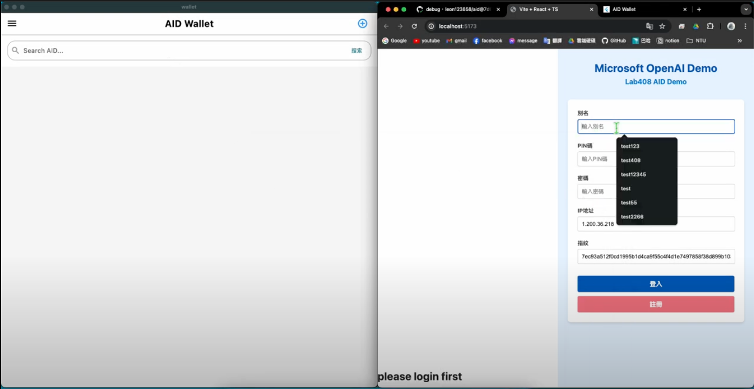
\includegraphics[width=\linewidth]{figures/AI-demo-logout.png}
  \caption{AI聊天軟體(未登入)}
  \label{fig:appendix-AI-demo-logout}
\end{figure}
\clearpage
\begin{figure}[p]
  \centering
  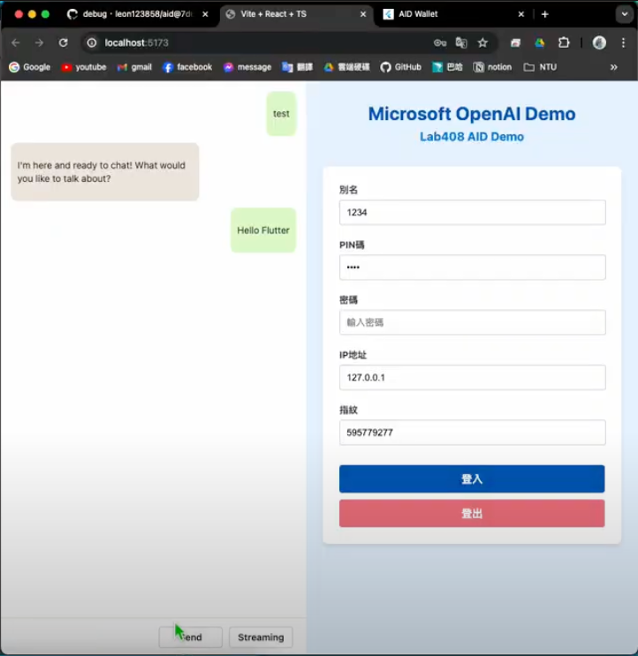
\includegraphics[width=\linewidth]{figures/AI-demo.png}
  \caption{AI聊天軟體(已登入)}
  \label{fig:appendix-AI-demo}
\end{figure}
本節展示實作部分的AI聊天軟體操作介面,使用者可以通過AID錢包登入並使用聊天功能。
\begin{itemize}
  \item 圖\ref{fig:appendix-AI-demo-logout}展示了AI聊天軟體的未登入狀態,使用者沒辦法使用聊天功能。
  \item 圖\ref{fig:appendix-AI-demo}展示了AI聊天軟體的已登入狀態,使用者可以通過AID錢包登入並直接聊天。
\end{itemize}
